\documentclass[11pt]{article}

\usepackage[utf8]{inputenc}
\usepackage[margin=1.25in]{geometry}
\usepackage{subcaption}
\usepackage{cite}
\usepackage{graphicx}
\usepackage[
  plainpages=false,
  pdfpagelayout=TwoPageRight,
  pdfborder={0 0 0},
  hyperfootnotes=false
]{hyperref}
\usepackage{amssymb}
\usepackage{amsmath}
\usepackage{caption} % For captioning tables and figures
\usepackage{array} % For more flexible table formatting
\usepackage{tabularx}
\usepackage{booktabs}
\usepackage{xcolor}
\usepackage{makecell}

\begin{document}

\begin{titlepage}
    \centering
    \includegraphics[width=0.2\textwidth]{assets/uni-logo.png}\par\vspace{0.5cm}
    {\scshape\LARGE Friedrich Schiller University, Jena \par}
    \vspace{1cm}
    {\scshape\Large Seminar Paper for Advanced Methods in Computer Vision\par}
    \vspace{1.5cm}
    {\huge\bfseries An Overview of the Inner Workings, Impacts, and Related Research of Stable Diffusion and Its Offsprings\par}
    \vspace{2cm}
    {\Large\itshape Phillip Rothenbeck, Lean Manthey, and Moritz Seppelt\par}
    \vfill
    supervised by\par
    M.Sc.~Niklas \textsc{Penzel}

    \vfill

    {\large \today\par}
\end{titlepage}

\tableofcontents
\newpage

\section{Introduction}
In recent years, the rise of text-to-image models has changed the way we approach the generation of images, allowing anyone to generate high-quality images from nothing more than text prompts. In this area, Stable Diffusion~\cite{rombach2022stablediffusion} has been a milestone model that advanced the field in terms of efficiency and quality in image generation. However, with the recent growing concerns over the computational cost, energy consumption, and control of the output, recent works such as Würstchen and ControlNet have come up with novel approaches to meet those challenges while maintaining or enhancing image quality. In this paper, we investigate Stable Diffusion, Würstchen~\cite{pernias2024wrstchen}, and ControlNet~\cite{zhang2023addingconditionalcontroltexttoimage} by discussing the architecture of each, re-implementing an experiment from their respective papers, and discuss their results. We also debate the greater social consequences of such technologies, particularly in light of developments in text-to-image AI.
\\
\\
\noindent
\textbf{Stable Diffusion} achieved its improvements in efficiency and quality by not generating images directly in the pixel space, which is computationally expensive. Instead, it performs its calculations in latent space, a more abstract representation of image data in which synthesis complexity is drastically lower. This shift enabled faster, more efficient image generation with no compromises in quality, hence, Stable Diffusion is one of the most important improvements from its earlier methods, for example GANs~\cite{dhariwal2021diffusionmodelsbeatgans}. By reducing the computational demands for image synthesis, Stable Diffusion has become one of the most used models, though it still requires substantial resources and Rombach et al.\ state, the training of SD 2.1~\cite{rombach2023sd_2_1} took around 200,000 GPU hours alone.
\\
\noindent
A more considerate alternative, when taking environmental and financial costs associated with such highly demanding models into count, is \textbf{Würstchen} by Pernias et al.\ Similar to Stable Diffusion, the backbone of Würstchen are LDMs. However, it makes critical changes with the aim of reducing computational load. Instead of generating images in one step, Würstchen splits the process into three phases, operating mainly in lower-dimensional latent spaces. This drastically reduces training time and computational cost and thus makes the approach more viable, without any sacrifice in image quality.
\\
\noindent
\textbf{ControlNet} brings further enhancements for diffusion-based models. Zhang et al.\ describe a technique for fine-grained control over image generation. While the text prompt may be sufficient for basic image synthesis, generating more complex layouts, poses, or even shapes is hard to achieve with text description only. ControlNet overcomes this limitation by providing conditional control to pre-trained diffusion models like Stable Diffusion. It does so by incorporating a secondary trainable network that handles additional inputs such as edge maps, human poses, or segmentation maps, giving users the ability to specify more detailed and accurate compositions. This flexibility further enhances the usability of diffusion models with more complex tasks, while keeping the robustness of the original model through its architecture, which locks the pre-trained layers while fine-tuning a trainable copy.
\\
\\
\noindent
We provide a deep dive into the technical details of each model, reproduce one experiment from each original research paper, and look into the results of these experiments to understand strengths and weaknesses for each approach. Also, we will consider wider implications for society in general, regarding text-to-image AI, including bias and ethics related to content creation associated with large-scale model training. In doing so, we try to give a picture of the current state of text-to-image AI, as well as future developments leading to a more sustainable and responsible development of the technology.

\section{Related Work}
\subsection{Stable Diffusion}
Before Stable Diffusion, generative models for image synthesis faced several challenges due to the high dimensionality of image data. Generative Adversarial Networks (GANs) \cite{goodfellow2014GAN} produced high-resolution images with strong perceptual quality \cite{bigganbrock, DBLP:journals/corr/abs-1912-04958} but were difficult to optimize and struggled to fully capture data distributions \cite{arjovsky2017wasserstein, gulrajani2017improved, DBLP:journals/corr/abs-1801-04406}. Likelihood-based methods such as Variational Autoencoders (VAEs) \cite{VAE} and flow-based models \cite{dinh2015nice, DBLP:conf/iclr/DinhSB17} improved density estimation and allowed efficient high-resolution synthesis \cite{DBLP:journals/corr/abs-2011-10650, glow, DBLP:conf/nips/VahdatK20}, but their sample quality lagged behind GANs. Autoregressive models (ARMs) \cite{DBLP:conf/icml/ChenRC0JLS20, DBLP:journals/corr/abs-1904-10509, NIPS2016_b1301141, DBLP:journals/corr/OordKK16}, while excelling in density estimation, were limited to low-resolution images due to computational complexity and sequential sampling requirements.

Diffusion Probabilistic Models (DMs) \cite{sohldickstein2015deepunsupervisedlearningusing} achieved state-of-the-art results in both density estimation \cite{kingma2023variationaldiffusionmodels} and sample quality \cite{dhariwal2021diffusionmodelsbeatgans}, benefiting from image-like data when paired with neural architectures like UNet \cite{dhariwal2021diffusionmodelsbeatgans, ronneberger2015unetconvolutionalnetworksbiomedical, DBLP:journals/corr/abs-2011-13456}. Despite their success, DMs trained on pixel space suffered from slow inference speeds and high training costs, even with advanced sampling strategies and hierarchical methods \cite{DBLP:journals/corr/abs-2106-15282, DBLP:journals/corr/abs-2106-00132, DBLP:journals/corr/abs-2104-02600, DBLP:conf/iclr/SongME21, DBLP:journals/corr/abs-2106-05931}.

Two-stage approaches \cite{DBLP:conf/iclr/DaiW19, esser2021tamingtransformershighresolutionimage, DBLP:conf/nips/RazaviOV19, DBLP:conf/nips/RombachEO20, DBLP:journals/corr/abs-2104-10157, yu2021vectorquantized} sought to combine the strengths of various generative models. For instance, VQ-VAEs \cite{DBLP:conf/nips/RazaviOV19, DBLP:journals/corr/abs-2104-10157} used ARMs over a discretized latent space, while VQGANs \cite{esser2021tamingtransformershighresolutionimage, yu2021vectorquantized} introduced adversarial and perceptual objectives to scale autoregressive transformers. However, these methods were limited by high computational costs and trade-offs between compression rates and image quality \cite{esser2021tamingtransformershighresolutionimage, ramesh2021zeroshottexttoimagegeneration}.


\subsection{W\"urstchen}
As latent diffusion models such as Stable
Diffusion~\cite{rombach2022stablediffusion} yield high image quality they come
with two disadvantages: the training time and the computational costs. Thus,
the need for a efficacy improvement arises. In this section, we present other
approaches for general diffusion models to solve this issue.

In 2020, Ho et al.~\cite{ho2020denoisingdiffusionprobabilisticmodels} introduced
the  denoising diffusion probabilistic model (DDPM) which yielded promising
results in generative modeling. Building on this work, Nichol et
al.~\cite{Nichol2021ImprovedDenoisingDiffusionProbabilisticModels} provide a
modification in order to improve training time and sample quality. For
instance, they proposed to use cosine-based noise schedules leading to a faster
convergence by distributing noise more effectively during training.
Furthermore, in contrast to DDPM they introduce learnable variances in the
reverse process, allowing the model to better capture uncertainties.

Furthermore, Zhang et al.~\cite{zhang2023fastsamplingdiffusionmodels} focus on the
improvement of sampling time and efficiency. To achieve this, they propose the
Diffusion Exponential Integrator Sampler (DEIS) to accelerate the reverse
diffusion process. By selectively training on masked portions of the data,
their approach reduces training iterations while preserving high-fidelity
samples, making diffusion models more efficient and scalable to larger
datasets.

In order to efficiently train large diffusion models, Zheng et
al.~\cite{zheng2024fast} introduce masked transformers. Their approach
selectively masks portions of the input data during training, enabling the
model to focus on reconstructing these masked regions. This selective training
reduces the amount of data processed in each iteration

W\"urstchen on the other hand, works in compact latent spaces in two-stage
generative process to reduce computational costs while also implementing
cosine-based schedules for the training of the C Stage (see
Section~\ref{sec:wuerstchen:training}) as the improved DDPM does.
\subsection{ControlNet}
This is the related work section for controlnet

\pagebreak
\section{Background}
\subsection{Stable Diffusion}
\label{heading:subsection:stable_diffusion}
In early 2022, computer scientists from LMU Munich and IWR Heidelberg proposed an improved approach to achieve high-resolution image synthesis\cite{rombach2022stablediffusion}. They called this method "latent diffusion models". It introduced the necessary performance boost to make the productive use and training of image models feasible on a large scale. But diffusion models were already known. The new idea was to generate a low-dimensional representation of the image by denoising and then upscaling it, instead of generating the full image by iterative diffusion. This small change was enough to achieve the required performance increase. Later, the descendant family of models was called "Stable Diffusion".

In this chapter, we will give an overview of the inner workings of stable diffusion, focusing on the text-to-image technique. It consists of three main parts:
\begin{enumerate}
    \item Text input is converted into conditioning vectors. This is done using a transformer architecture.
    \item The main step is iterative denoising. Here, the conditioning vectors influence the resulting latent representation. A neural network called U-net does the heavy lifting.
    \item Finally, the latent representation must be converted into the final image. This is done using an auto-decoder.
\end{enumerate}

Let's assume that all machine learning components already have their trained weights and biases. Equipped with these, we will go through step by step how a text input is transformed into an image. After that, the training process is presented.

\subsubsection{Conditioning}
For stable diffusion, the conditioning process is a series of different existing components that are plugged together with the goal of semantically understanding the input prompt. First, the input sentence is tokenized. They used the BERT tokenizer\cite{devlin2019bert}. Basically, tokenization means breaking the input into small pieces called tokens. These tokes can be thought of as words or parts of words.

Second, these tokens are embedded in a Euclidean vector space. This already encodes some semantic meaning. Tokens that have similar meanings are mapped to vectors that point to approximately the same region in this high-dimensional space. For example, the words "achieve" and "accomplish" would be closer than "achieve" and "annoying". But even more, directions or distances can be interpreted. This could be thought of as relations between words. For example, the embedding of "Germany" and "Berlin" is expected to have the same distance as "Spain" and "Madrid".

This simple representation is not enough to understand the input. The meaning of words changes drastically depending on the surrounding words. To quote the English linguist J. R. Firth \textit{You shall know a word by the company it keeps}\cite{firth1962studiesinlinguisticanalysis}. To capture these important relationships, the creators of Stable Diffusion used the so-called cross-attention algorithm\cite{vaswani2023attentionneed}. It adapts the embeddings by selectively attending to other relevant tokens in the sequence, thereby incorporating contextual information. This allows the embeddings to more accurately capture the relationships between words, ensuring that the model's understanding of each token is enriched by its surrounding context.


\iffalse
    It operates by computing three different vectors for each token in the input sequence for each type of relationship there could be in the sentence: the Query ($Q$), the Key ($K$), and the Value ($V$) vectors. These vectors are derived from the embedded token vectors through linear transformations, which are essentially matrix multiplications with learned weight matrices. Specifically, for each token, we calculate:
    $$Q = X \cdot W_Q,\quad K = X\cdot W_K,\quad V = X \cdot W_V$$
    Where $X$ is the matrix of embedded token vectors, and $W_Q$, $W_K$ and $W_V$ are learned weight matrices for the Query, Key, and Value, respectively.

    Once we have the Query ($Q$), Key ($K$), and Value ($V$) vectors for each token, the next step is to determine how much each token should focus on the others. The goal here is to figure out which other words in the sentence are most relevant to the current word, given the context.
    Imagine each Query vector as a question that each word is asking about its context. The Key vectors, on the other hand, represent the possible answers that other words can provide. The dot product between a Query and a Key is like measuring how well the question matches the answer. If the Query and Key vectors are similar, it means that the word being asked about is highly relevant to the current word, and so it should be paid more attention.
    However, to prevent these dot products from getting too large when working with high-dimensional vectors, we scale them down by the square root of the Key vector's dimension, $\sqrt{d_k}$.

    $$\frac{QK^\top}{\sqrt{d_k}}$$

    Next, we convert these scaled dot products into attention scores using a softmax function. The softmax function turns these scores into probabilities, where higher scores mean more attention should be given to that token. For example, if "Harry" is the current word, and its Query vector strongly matches the Key vector of "wizard", the attention mechanism will assign a high probability to "wizard", meaning that "Harry" will focus more on "wizard" in this context.

    $$\mathrm{Attention Weights} = \mathrm{softmax}\left(\frac{QK^\top}{\sqrt{d_k}}\right)$$

    Finally, these attention scores are used to compute a weighted sum of the Value vectors. The Value vectors represent the actual information or content associated with each token. The weighted sum allows the model to combine the most relevant pieces of information from the other words, creating a new, context-aware representation of the current word.

    $$\mathrm{Output} = \sum_i \mathrm{Attention Weights}_i \cdot V_i$$

    This described process is done using many Key, Query and Value matrices to capture a how range of possible influences words can have on others. The output are context aware token embeddings.
\fi

\subsubsection{Iterative Denoising}
Iterative denoising is the crucial step in image generation. Remember, the goal is to generate a latent representation of the final image, which can be thought of as a low-dimensional representation, or just a smaller image. We start with random noise in this reduced size. Typically, this would be just a random sample from a Gaussian distribution. The goal will then be to gradually remove the noise to obtain clear, detailed images that match the description from the prompt.

It starts with a noised image, denoted as $x_T$, where $T$ is the total number of steps in the reverse diffusion process. Then the model uses a neural network which is trained to evaluate the function $\varepsilon_\theta(x_t,t,c)$ that estimates the noise at the current noised image $x_t$, $0 \leq t \leq T$ in each step, $c$ is the conditioning input. By approximating the current noise, we can just remove the noise, to slightly denoise the image.
$$x_{t-1}=x_t-\alpha_t \varepsilon_\theta(x_t,t,c)+ \alpha_t z_t$$
where $\alpha_t$ controls the step size for noise removal, and $\alpha_t z_t$  ($z_t$ is some Gaussian noise) adds controlled noise to maintain some stochasticity. This update moves the noisy image closer to a cleaner version, progressively refining it. This step is performed $T$-times, and at $t=0$ we arrived at a denoised latent representation of the final image.

\paragraph{U-Net}
One might wonder, how we calculate $\varepsilon_\theta(x_t,t,c)$ and thus approximate the current noise. This is done using a neural network architecture called U-Net\cite{ronneberger2015unetconvolutionalnetworksbiomedical}, that is well-suited for tasks where you need to transform one image into another, as is needed here.
The U-Net architecture gets its name from its distinctive "U" shape (see fig. \ref{fig:unet}), which reflects the way the network processes information. The U-Net consists of two main parts: the downsampling path and the upsampling path, connected by a bottleneck in the middle.
In the downsampling path, the U-Net gradually reduces the image size while capturing important features. Once the image reaches the bottleneck, it has been compressed into a highly abstract representation. This is where the most essential features are concentrated, and it serves as the transition point between the downsampling and upsampling paths. The upsampling path then constructs the resulting image, restoring the original size and adding details. Skip connections between corresponding layers in these paths help preserve fine details by directly passing information from the encoder to the decoder.
The result is then the approximated noise at this stage of the denoising process, which can be further used, as described above.

\begin{figure}[h]
    \centering
    \includegraphics[width=0.4\textwidth]{assets/u-net-illustration-correct-scale2.pdf}
    \caption{Depiction of U-Net architecture (example for 32x32 pixels in the lowest resolution). Image Source \cite{ronneberger2015unetconvolutionalnetworksbiomedical}}
    \label{fig:unet}
\end{figure}

\subsubsection{Decoder}
The last part involves converting the latent representation of an image into the output image. As the latent representation is of lower dimensionality, we need to find a way to add detail. To achieve this, the decoder typically employs a series of upsampling and convolutional layers. These layers progressively increase the spatial dimensions of the latent representation while refining the details at each step. The process is analogous to zooming in on a blurred thumbnail, but with the added capability of restoring fine details based on the encoded information.
Throughout this process, the decoder leverages the rich information captured in the early stages of the model, ensuring that the final image not only fits the structure implied by the latent representation but also accurately reflects the content described by the input prompt. The end result is a high-quality, detailed image that visually matches the semantics of the original text input.


\subsubsection{Training}
\label{sec:stabel_diffusion:training}
In the previous sections, we explored a variety of machine learning components that are integral to achieving text-to-image generation capabilities with models like Stable Diffusion. Specifically, these components include the tokenizer, embeddings, transformer (comprising value, query, and key matrices), the U-Net, and the decoder. Pretrained weights are typically used for the tokenizer, word embeddings, and transformer. However, the U-Net, which predicts the noise in the denoising process, and the decoder, which converts the latent representation into the final image, typically require dedicated training. In this chapter, I will focus on the structure of the training data and the loss functions employed in training these components. Although detailed optimization algorithms and mathematical derivations are beyond the scope of this discussion, a comprehensive understanding begins with the decoder and works backward through the model pipeline.

\paragraph{Training the Decoder}
To effectively train the decoder, we introduce an additional component, the encoder, which is crucial for training but not needed during inference. The encoder maps an input image to its corresponding latent representation, forming a Variational Autoencoder (VAE)\cite{kingma2022autoencodingvariationalbayes} together with the decoder. The VAE is a generative model that learns a compressed representation of data in a latent space, balancing the trade-off between reconstruction fidelity and latent space regularization. The encoder and decoder are trained jointly to minimize a loss function that comprises two key terms:

The reconstruction loss $\mathcal{L}_{\mathrm{reconstruction}}$ measures the fidelity of reconstruction. After encoding an image into its latent representation, the decoder attempts to reconstruct the original image from this representation. The reconstruction loss is typically the mean squared error (MSE) between the original and reconstructed images, encouraging the model to learn latent representations that allow for accurate reconstructions.

To prevent the latent space from becoming arbitrarily dispersed and to encourage smooth transitions between points in the latent space, a regularization term based on the Kullback-Leibler (KL) divergence~\cite{kullback1951OnInformationandSufficiency} is added. The KL divergence measures how much the distribution of latent variables deviates from a predefined prior distribution, often using a standard normal distribution. By minimizing this divergence, the VAE ensures that the latent space is well-structured and that similar images map to nearby points in the latent space. We arrive at the formula:

$$\mathcal{L}_{\mathrm{VAE}} = \mathcal{L}_{\mathrm{reconstruction}} + \beta \mathcal{L}_{\mathrm{KL}}$$
where $\beta$ is a coefficient to control the trade-off between reconstruction fidelity and latent space regularization.

Once trained, the VAE can be used to generate latent representations of images, which are essential for the subsequent training of the U-Net, which we will explore now:

\paragraph{Training the U-Net}
With the trained VAE, the next step is to train the U-Net, a critical component in the denoising process. The U-Net is trained within the framework of a Denoising Diffusion Probabilistic Model (DDPM)\cite{ho2020denoisingdiffusionprobabilisticmodels}, a generative model that iteratively refines a noisy image to recover the underlying clean image. The training process for the U-Net proceeds as follows.

Begin with a labeled dataset of images. In the case of Stable Diffusion, the ImageNet dataset~\cite{deng2009imagenet} was used. Each image is passed through the trained encoder of the VAE to obtain its latent representation. This latent space has lower dimensionality than the original image space, increasing the computational efficiency of the learning process.

Gaussian noise is added to the latent representation of an image over multiple time steps, ultimately transforming it into a distribution of pure noise. This sequence of increasingly noisy images, referred to as Forward Diffusion, constitutes the training data for the U-Net.

The primary task of the U-Net is to predict the noise that was added to a given noisy image. For each time step, the U-Net takes as input the noisy image and a conditioning vector derived from the text label using the pretrained transformer. It then predicts the noise component that was added during the forward diffusion process. The actual noise component is computed as the difference between consecutive noisy images in the sequence.

The training objective is defined as the mean squared error (MSE) between the predicted noise and the actual noise. By minimizing this loss, the U-Net learns to accurately estimate the noise at each step. This enables it to reverse the diffusion process during inference, effectively denoising the image and recovering the clean latent representation.

\subsection{W\"urstchen}
In Section~\ref{heading:subsection:stable_diffusion}, we describe the approach
of a \emph{Latent Diffusion Model} (LDM) which was introduced,
by Rombach et al.~\cite{rombach2022stablediffusion} in 2022. The LDM methods
generate images by denoising a noisy latent image gradually step by step. To
conduct the reduction of noise and the introduction of semantics, the LDM takes
in an encoding of a text-prompt, called token or embedding, and utilizes it for
each diffusion step. Lastly, the latent representation is decoded into the
pixel space. By mostly navigating in low dimensional latent spaces and
using the U-Net to gradually introdue semantics into the representation, this
approach is able to yield high resolution images~\cite{rombach2022stablediffusion}.
This improvement in image quality has a disadvantage: the time the models take
to train. For example, an important model is Stable Diffusion (SD), the version
1.4 takes 150,000 GPU hours~\cite{rombach2022sd_1_4} while version 2.1 which
grants an upgrade in image quality has a further increased training time of
200,000 GPU hours~\cite{rombach2023sd_2_1}. A high image resolution comes with
an increased image complexity leading to more data-intensive training and
high computational costs. Thus, Pernias et al.~\cite{pernias2024wrstchen}
introduce \emph{W\"urstchen}. An approach that aims to decrease the training
time and computational cost, by splitting the training process into three parts
and mostly computing in small latent spaces.

This section aims to describe the methods used by W\"urstchen based on the work
of Pernias et al.~\cite{pernias2024wrstchen}. First, we describe the VQGAN by
Esser et al.~\cite{esser2021tamingtransformershighresolutionimage} as this is
the model that is the foundation for Stage A of W\"urstchen. Then, we continue
to shed light onto the general structure and the image generation process. Finally, we
describe the training processes of each W\"urstchen stage as Pernias et al.
provide them.
\subsubsection{VQGAN}
\label{sec:wuerstchen:VQGAN}
The \emph{Vector Quantized Generative Adversarial Network} (VQGAN) was
introduced by Esser et al.~\cite{esser2021tamingtransformershighresolutionimage}
in 2021 and builds on the \emph{Vector Quantized Variational Autoencoder}
model~\cite{vdOord2017NeuralDiscreteRepresentationLearning}. The VQGAN combines
the strengths of \emph{Convolutional Neural Networks} (CNNs) in exploiting local 
features and the strength of autoregressive transformer architectures
to model long-range relations in generated images. Esser et al. introduce
several CNNs to the VQGAN for the training procedure. First, the Encoder CNN
compresses an image $x$ into the compressed version $\hat{z}$. Next,
the VQGAN utilizes the quantization $\boldsymbol{q}[\cdot]$ using a
perceptually rich and discrete codebook $\mathcal{Z}$ to create the quantized
latent representation,
\begin{equation}
    z_{\boldsymbol{q}} = \boldsymbol{q}(\hat{z}) :=\underset{z_{\boldsymbol{k}}\in\mathcal{Z}}{\arg\min}||\hat{z}_{ij} - z_{\boldsymbol{k}}||,
\end{equation}
by replacing the spatial representation $\hat{z}_{ij}$ with the closest
codebook entry $z_{\boldsymbol{k}}$. The latent representation
$z_{\boldsymbol{q}}$ is a sequence of the entries of the codebook $\mathcal{Z}$.
Then, the Decoder CNN reconstructs the image $x$ using the quantized latent
representation $z_{\boldsymbol{q}}$. Finally, to create a rich codebook
a patch-based discriminator CNN is introduced to find the differences between
the real and reconstructed images. An autoregressive transformer model then
makes use of the codebook to generate high-resolution synthetic images.
\subsubsection{W\"urstchen Structure and Image Generation}
\begin{figure}[t]
    \includegraphics[width=\textwidth]{assets/wuerstchen_arch.pdf}
    \caption{Visualization of the W\"urstchen architecture, introduced by
        Pernias et al.~\cite{pernias2024wrstchen}. It shows that the first stage C
        creates a highly compressed representation from noise and text-conditioning.
        Both this representation and the text-prompt are then utilized as conditionings by stage B
        to create a higher dimensional latent representation. Lastly, the decoder
        in stage A generates an image from this latent representation.}
    \label{fig:wuerstchen:arch}
\end{figure}
In 2024, Pernias et al.~\cite{pernias2024wrstchen} introduce \emph{W\"urstchen}.
With this method, they aim to decrease the computational cost and training
time of image generation models which are based on latent diffusion~\cite{rombach2022stablediffusion}.
Figure~\ref{fig:wuerstchen:arch} illustrates the structure of W\"urstchen which
includes three stages. The first stage, Stage C, comprises a
text-conditional diffusion model $f_\Theta$ that operates on a low-dimensional
latent space with a compression ratio of 42:1. In this stage, the image generation 
pipeline begins by taking latent random noise
$\boldsymbol{X}_{\text{SC}, \tau_C} = \mathcal{N}(0, \boldsymbol{\text{I}})$ and
using the DDPM algorithm by Ho et al.~\cite{ho2020denoisingdiffusionprobabilisticmodels} to iteratively
sample the Semantic Compressor (see Section~\ref{sec:wuerstchen:training})
latent representations on text-conditioning to generate the latent representation
$\bar{\boldsymbol{X}}_{\text{SC}}\in\mathbb{R}^{16\times24\times24}$. Due to
the low dimensionality of the latent space, $f_\Theta$ does not utilize the
typical U-Net structure as the authors decided that any downsampling would do
harm to the image quality. The next stage, Stage B, employs a diffusion model
$f_\vartheta$, utilizing the U-Net architecture. It is conditioned on both the
text-prompt and the embeddings $\mathcal{C}_{\text{SC}}$ of the flattened
$\bar{\boldsymbol{X}}_{\text{SC}}$ from Stage C. This model generates a
higher-dimensional latent representation
$\tilde{\boldsymbol{X}}\in\mathbb{R}^{4\times256\times256}$ by again employing
the DDPM algorithm. The latent space in which $\tilde{\boldsymbol{X}}$ lives
has a compression ratio of 4:1 and is created during the training process by a
VQGAN. Stage A of W\"urstchen consists of the decoder $f_\Theta^{-1}$ which is
part of the same VQGAN. The decoder translates the latent representation
$\tilde{\boldsymbol{X}}$ to the final image,
\begin{equation}
    \bar{\boldsymbol{X}} = f_\Theta^{-1}(\tilde{\boldsymbol{X}}),
\end{equation}
which lives in the pixel space with $\bar{\boldsymbol{X}}\in\mathbb{R}^{3\times1024\times1024}$.
Pernias et al. train each of these stages separately, which we describe in the
following section.
\subsubsection{Training}
\label{sec:wuerstchen:training}
The preceding section provides an overview of the architecture and structure
of W\"urstchen.
In order to train the model in a more efficient manner, Pernias et
al.~\cite{pernias2024wrstchen} introduce a split-training approach. This enables
them to mainly train in low-dimensional latent spaces, which leads to
performance improvements. Pernias et al. perform the training in reverse order
from the image generation process (see Figure~\ref{fig:wuerstchen:arch}).
The reason for this are the dependencies between Stage A and Stage B, and Stage B and Stage C.
First, they train Stage A which defines the latent space (4:1) through its VQGAN.
Following this, Stage B learns to reconstruct this latent space using embeddings in a
lower dimensional latent space (42:1) which are produced by a semantic compressor.
Finally, Stage C trains to reconstruct the latent space of the semantic
compressor using text-conditioning. The following paragraphs shed light on the methods
of Pernias et al. in greater detail.
\begin{figure}[t]
    \includegraphics[width=\textwidth]{assets/wuerstchen_training.pdf}
    \caption{Visualization of the training processes of each W\"urstchen stage~\cite{pernias2024wrstchen}.
        On top the training of Stage A followed by Stage B and finally by stage C.
        The training processes of Stages B and C utilize diffusion losses while
        Stage A is trained as a VQGAN.}
    \label{fig:wuerstchen:training}
\end{figure}

\paragraph*{Stage A} The last stage in the image generation pipeline consists of a decoder
$f_{\Theta}^{-1}$ and translates the latent representation produced by Stage B into
the pixel space. This decoder is part of a VQGAN and Pernias et al. train it as
Esset et al.~\cite{esser2021tamingtransformershighresolutionimage} describe.
We touch on this process in Section~\ref{sec:wuerstchen:VQGAN}. During training,
first an encoder $f_{\Theta}$ compresses an image $\boldsymbol{X}\in\mathbb{R}^{3\times1024\times1024}$. Then the compressed image is
quantized using a codebook yielding a latent representation $\boldsymbol{X}_q\in\mathbb{R}^{4\times256\times256}$ of the image with,
$\boldsymbol{X}_q = f_{\Theta}(\boldsymbol{X}).$
Finally, the decoder $f_{\Theta}^{-1}$ reconstructs the image from the latent.
The decoder and encoder are supposed to fulfill the equation,
\begin{equation}
    f_{\Theta}^{-1}(f_{\Theta}(\boldsymbol{X})) = f_{\Theta}^{-1}(\boldsymbol{X}_q) \approx \boldsymbol{X}.
\end{equation}
During training the encoder, the decoder and the codebook are defined. The
encoder defines the latent space with a 4:1 compression ratio, which is
the codomain of the next stage.

\paragraph*{Stage B} This stage reconstructs the latent space defined by the
VQGAN in the training process of Stage A. Therefore, the encoder $f_{\Theta}$
is used to compress the image but without the quantization from the preceding stage.
After noising, the representation $\tilde{\boldsymbol{X}}_t\in\mathbb{R}^{4\times1256\times256}$
is given to the model $f_\vartheta$. For
conditioning Stage B uses both the text embeddings and the results of a
\emph{semantic compressor} $e_{\Phi}$. This semantic compressor mimics Stage C and will be
the foundation of Stage C's training process.

The semantic compressor is a feature extractor of any kind that is supposed to
compress an image to a high degree. The authors advise to choose a model with a
good feature representation and small network size in order to fasten the training
precess of both Stages B and C. Additionally, they mention the size of the
feature space, as too few dimensions would lead to a loss of detail, while to
many dimensions can have a great impact on the computation costs and time. For
these reasons, Pernias et al. chose the CNN, ImageNet1k pre-trained EfficientV2 (S)~\cite{Tan2021EfficientNetV2}.
The semantic compressor gets a bicubic interpolated version of the image and
produces its highly compressed version. Afterward, a $1\times1$ convolution is
applied to reduce the depth and further compress the latent representation $\mathcal{C}_{\text{SC}}\in\mathbb{R}^{16\times24\times24}$.

The embeddings $\mathcal{C}_{\text{SC}}$ of the semantic compressor and the
text-conditioning $\mathcal{C}_{\text{text}}$ are both implemented into the training process using Cross-Attention~\cite{vaswani2023attentionneed}.
Pernias et al. add noise to $\mathcal{C}_{\text{SC}}$ and randomly drop it to
sample with classifier-free-guidance~\cite{ho2022classifierfreediffusionguidance}.
Using both the noised latent representation of the encoder $f_\Theta$ and the
conditioning, the model $f_\vartheta$ trains with the standard diffusion
procedure as we discuss in Section~\ref{sec:stabel_diffusion:training}.

\paragraph*{Stage C} The last stage is supposed to reconstruct the latent space
defined by the semantic compressor $e_\Phi$. Thus, the embeddings
$\mathcal{C}_{\text{SC}}$ are generated as explained for Stage B. Pernias et
al. add a weighted noise to the latent representation
$\boldsymbol{X}_{\text{SC}} = \mathcal{C}_{\text{SC}}$ generated by $e_\Phi$,
\begin{equation}
    \boldsymbol{X}_{\text{SC}, t} = \sqrt{\bar{\alpha}_t}\cdot\boldsymbol{X}_{\text{SC}}+\sqrt{1-\bar{\alpha}_t}\cdot\epsilon,
\end{equation}
with $\bar{\alpha}_t$ defined by a cosine schedule~\cite{Nichol2021ImprovedDenoisingDiffusionProbabilisticModels}.
The model takes $\boldsymbol{X}_{\text{SC}, t}$, $\mathcal{C}_{\text{text}}$ and
the time step $t$ as an input and predicts the error,
\begin{equation}
    \bar{\epsilon} = \frac{\boldsymbol{X}_{\text{SC}, t} - \boldsymbol{A}}{|1-\boldsymbol{B}| + 1e^{-5}} \quad \text{with} \quad \boldsymbol{A}, \boldsymbol{B} = f_\Theta(\boldsymbol{X}_{\text{SC}, t},\mathcal{C}_{\text{text}}, t).
\end{equation}
As the authors mention, they found this change of objective to yield a more
stable training process. The text-embeddings are produced using
CLIP-H~\cite{Ilharco2021OpenCLIP} and are dropped 5\% of the times. In the same
way as the Stage B model, the model $f_\Theta$ is trained using the diffusion
procedure, while conditioning is applied after each block using cross-attention.
\subsection{ControlNet}
In 2023, Lvmin Zhang, Anyi Rao and Maneesh Agrawala from the Stanford University introduced a method for adding conditional control to text-to-image diffusion models~\cite{zhang2023addingconditionalcontroltexttoimage}. They dubbed this neural network architecture ``ControlNet''. ControlNet adds conditional control to pretrained neural network blocks by incorporating a secondary, trainable network. The process involves freezing the parameters of the original model blocks (e.g., ResNet or transformer blocks) and creating a trainable copy that receives external conditioning vectors. We first describe the basic architecture of ControlNet and a more concrete example of how Zhang et al.\ applied it to Stable Diffusion, followed by the training of ControlNet. Lastly, we discuss some things to be noted for inference like classifier-free guidance resolution weighting and how to combine multiple conditions. 

\subsubsection{Architecture}
ControlNet's functioning can be described by looking at what happends to the individual network blocks. Let $\mathcal{F}(\cdot; \Theta)$ be a neural block with parameters $\Theta$ that transforms an input feature map $x$ into an output feature map $y$:
\[
y = F(x; \Theta).
\]
\noindent
To integrate ControlNet, the parameters $\Theta$ of the original block are frozen/locked, and the block is cloned into a trainable copy with new parameters $\Theta_c$, as seen in Figure~\ref{fig:control_net:network_blocks}. The copy also takes an external conditioning vector $c$ as input. This configuration preserves the original model's robust capabilities while allowing the trainable copy to handle the input conditions.
\begin{figure}
    \centering
    \includegraphics[width=0.7\textwidth]{assets/control_net_network_blocks.pdf}
    \caption{A visualization from Zhang et al.~\cite{zhang2023addingconditionalcontroltexttoimage} of a neural block that takes a feature map $x$ as input and outputs another feature map $y$, as shown in (a). The ControlNet is added by locking the original block and create a trainable copy. They are connected using zero convolution layers with both weight and bias initialized to zero. The conditioning vector $c$ is added to the network, as shown in (b)}
    \label{fig:control_net:network_blocks}
\end{figure}
The trainable copy is connected to the original block via zero convolution layers, denoted as $Z(\cdot; \cdot)$. These are $1 \times 1$ convolutions initialized with zero weights and biases, ensuring no interference at the start of training. ControlNet uses two such zero convolutions, with parameters $\Theta_{z1}$ and $\Theta_{z2}$. The complete computation in ControlNet is defined as:
\[
y_c = \mathcal{F}(x; \Theta) + \mathcal{Z}(\mathcal{F}(x + \mathcal{Z}(c; \Theta_{z1}); \Theta_c); \Theta_{z2}),
\]
where $y_c$ is the output of the ControlNet block. Initially, due to zero-initialization of the convolutions, $\mathcal{Z}(\cdot; \cdot)$ evaluates to zero, simplifying the equation to:
\[
y_c = y.
\]
This ensures that noise does not affect the neural network's hidden states during early training. As $\mathcal{Z}(c; \Theta_{z1}) = 0$, the trainable copy operates with the original input $x$, preserving the pre-trained model's functionality while serving as a reliable backbone for further learning. Zero convolutions effectively shield the backbone from random noise in the initial gradients, supporting stable training from the start. This method allows ControlNet to utilize the strengths of large-scale pretrained models effectively, applying them to diverse conditions without the risk of catastrophic forgetting or degradation of the pretrained model's performance. 

\subsubsection{Adding ControlNet to Stable Diffusion}
We demonstrate Zhang et al.'s integration of ControlNet with a large pretrained diffusion model using Stable Diffusion~\cite{rombach2022stablediffusion}. Stable Diffusion is structured as a U-Net~\cite{ronneberger2015unetconvolutionalnetworksbiomedical} comprising an encoder, a middle block, and a skip-connected decoder. The encoder and decoder each consist of 12 blocks, and the entire model has 25 blocks, including the middle block. Of these 25 blocks, 8 are down-sampling or up-sampling convolution layers, and the remaining 17 are main blocks, each containing 4 ResNet layers and 2 Vision Transformers (ViTs). Each ViT includes cross-attention and self-attention mechanisms. For example, in Figure~\ref{fig:control_net:sd_architecture}a, the ``SD Encoder Block A'' comprises 4 ResNet layers and 2 ViTs, and the ``$\times$3'' notation indicates this block repeats three times. Text prompts are encoded using the CLIP text encoder~\cite{radford2021learningtransferablevisualmodels}, and diffusion timesteps are encoded with a positional time encoder.
\begin{figure}
    \centering
    \includegraphics[width=0.7\textwidth]{assets/control_net_sd_architecture.pdf}
    \caption{A simplified description used in ``Adding Conditional Control to Text-To-Image Diffusion Models''~\cite{zhang2023addingconditionalcontroltexttoimage} to explain ControlNet's architecture in conjunction with Stable Diffusion.}
    \label{fig:control_net:sd_architecture}
\end{figure}
ControlNet is applied to each encoder level of the U-Net, as seen in Figure~\ref{fig:control_net:sd_architecture}b. Specifically, ControlNet creates trainable copies of the 12 encoding blocks and 1 middle block from Stable Diffusion. The 12 encoding blocks are distributed across 4 resolutions (64~$\times$~64,~32~$\times$~32,~16~$\times$~16,~8~$\times$~8), with each resolution level replicated three times. The outputs are added to the 12 skip-connections and 1 middle block of the U-Net. Given that Stable Diffusion follows a typical U-Net architecture, this ControlNet configuration can be extended to other models. ControlNet is computationally efficient since the frozen parameters do not require gradient computation during fine-tuning, reducing the load on the locked encoder. This approach accelerates training and conserves GPU memory. Zhang et al.\ report that, on a single NVIDIA A100 PCIE 40GB, optimizing Stable Diffusion with ControlNet uses about 23\% more GPU memory and 34\% more time per training iteration than without ControlNet.

Image diffusion models learn by progressively denoising and generating samples within the training domain, which can occur in pixel space or latent space. In Subsection~\ref{heading:subsection:stable_diffusion}, we explained the inner workings of Stable Diffusion and its operation in the latent space. It preprocesses 512 $\times$ 512 images into 64 $\times$ 64 latent representations. To add ControlNet, input conditioning images (e.g., edges, poses, depth) of size 512 $\times$ 512 are converted to a matching 64 $\times$ 64 feature space using a small encoder network $E(\cdot)$ composed of four convolution layers with 4 $\times$ 4 kernels and 2 $\times$ 2 strides, activated by ReLU and using channels [16, 32, 64, 128]. These layers are initialized with Gaussian weights and trained alongside the full model. The resulting feature space conditioning vector $c_f$ is computed as:
\[
c_f = E(c_i),
\]
where $c_i$ is the input condition, and $c_f$ is passed into the ControlNet.

\section{Training}




\newpage
\section{Experiments}
Here our goal was, to test the reproducibility of the selected papers. Since it is computationally not feasible to reproduce every result, we selected one experiment per paper to review. For Stable Diffusion, we investigate the reproducibility and meaningfulness concerning Rombach et al.'s utilized metric. Second, for W\"urstchen, we state the hypothesis that the human perception of the generated images is generally worse than the reported results of Pernias et al.\ and conduct an experiment to proof this hypothesis. Last, to reproduce Zhang et al.'s experiment, we use ControlNet to generate images from sketches and compare it to other methods by performing a user study to obtain an average user ranking per method.

\subsection{The FID of Stable Diffusion}
\subsubsection{Selection of the experiment and background}
\label{sec:experiments:stabel_diffusion:selction_of_fid}
Before looking closer at the kinds of experiments conducted by the Stable Diffusion team, it was clear that we could not reproduce any training-related experiments, as these are generally computationally very expensive. The evaluation metrics appeared more promising, as certain scores were compared with the state-of-the-art models. Most notably, the FID-Score, which was calculated across different datasets.

The FID (Fréchet Inception Distance)\cite{heusel2018ganstrainedtimescaleupdate} score is a metric for evaluating the quality of images generated by generative or text-to-image models. It compares the distribution of generated images with the distribution of real images, providing a measure of how similar the generated images are to the real ones. The FID score calculates the Fréchet distance between two multivariate Gaussian distributions, one representing the features of real images and the other representing the features of generated images. These features are typically extracted using a pre-trained Inception v3 model. If $P_r$ is the distribution of the real images and $P_g$ is the distribution of the generated images, with $\mu_p, \mu_g$ as the respective means and $\Sigma_p, \Sigma_g$ the respective covariance matrices, than the FID score can be calculated as:
$$\mathrm{FID}(P_r, P_g) = \Vert\mu_r - \mu_g\Vert_2^2 + \mathrm{Tr}\left(\Sigma_r + \Sigma_p - 2 (\Sigma_r\Sigma_g)^\frac{1}{2}\right)$$
A lower FID Score indicates that the generated images are more similar to real images, implying higher quality, while a higher FID Score suggests a greater discrepancy between the distributions of real and generated images, indicating lower quality.

Upon analyzing the paper, we noticed that a different rendering of Stable Diffusion was used depending on the dataset. The parameters that were changed mostly included the dimensionality of the latent space and the number of diffusion steps. This seems odd, as it may suggest that the researchers were cherry-picking the best possible results. Additionally, a hypothesis test was omitted, which would have made reproducing these experiments more useful and interesting. This may also indicate that the results were not simply due to chance.

\subsubsection{Experiment description and methodology}
As the text-to-image capabilities of Stable Diffusion were our main focus, we chose to reproduce the "Text-Conditional Image Synthesis" experiment from the original paper. In that experiment, the FID score based on the MS-COCO validation dataset\cite{lin2015microsoftcococommonobjects} was calculated and compared against the result of other state-of-the-art text-to-image models at the time. As described above, a specific version of Stable Diffusion was chosen to achieve this result. In this case, $250$ diffusion steps were used, along with an $8$ times smaller latent space. The paper provided a FID score of $23.31$.

The experiment proceedes as follows. For each image in the dataset, we get its caption and use it to generate an image with Stable Diffusion. This allows us to reproduce the images in the MS-COCO validation dataset. Afterward, we scale the images so that they all have the same dimensions. We selected dimensions of $299\times299$. Finally, we use \texttt{torch-fidelity}\cite{obukhov2020torchfidelity} by PyTorch to calculate the FID score. This process is repeated for the different numbers of diffusion steps.

\subsubsection{Results}
\begin{table}[hbp]
    \centering
    \caption{Comparison of FID score of the paper and other models with our results}
    \label{tab:fid_is_comparison}
    \begin{tabular}{lc}
        \toprule
                                                                               & \textbf{FID} \\
        \midrule
        \textbf{Original Paper}                                                & $23.31$      \\
        \textbf{Our result}                                                    & $24.56$      \\\addlinespace
        CogView \cite{ding2021cogviewmasteringtexttoimagegeneration}           & $27.10$      \\
        LAFITE \cite{zhou2022lafitelanguagefreetrainingtexttoimage}            & $26.94$      \\
        GLIDE \cite{rezende2014stochasticbackpropagationapproximateinference}  & $12.24$      \\
        Make-A-Scene \cite{gafni2022makeascenescenebasedtexttoimagegeneration} & $11.84$      \\
        \bottomrule
    \end{tabular}
\end{table}

As shown in Tab. \ref{tab:fid_is_comparison}, the FID score is slightly worse. However, since error bounds for the FID score were not provided and no hypothesis testing was performed, it is challenging to evaluate this outcome. The metrics for the other image-generating models are the same ones that Stable Diffusion was compared to in the original paper. We can observe that Stable Diffusion's ranking did not change when using our metrics within the provided examples.

Nonetheless, there is a significant difference between the FID scores. This discrepancy may arise from various factors: differences in the calculation pipeline, e.g. by a more modern version of \texttt{torch-fidelity}, randomness in the generated image data or slightly different preprocessing methods.

\subsubsection{Stability of the FID score}
\begin{figure}
    \centering
    % First subfigure: The plot you created
    \begin{subfigure}{0.49\textwidth}
        \includegraphics[width=\textwidth]{assets/num_samples_comparison.pdf}
        \caption{FID scores for datasets in different sizes.}
        \label{fig:num_samples_comparison}
    \end{subfigure}
    \hfill
    % Second subfigure: The PDF file 'num_samples_comparison_corrected.pdf'
    \begin{subfigure}{0.49\textwidth}
        \includegraphics[width=\textwidth]{assets/num_samples_comparison_corrected.pdf}
        \caption{Graph of proposed corrected FID score.}
        \label{fig:num_samples_comparison_corrected}
    \end{subfigure}
    \caption{Comparison of FID scores across different sample sizes. Here, subsets of MS-COCO where used with 250 diffusion steps.}
\end{figure}

In general, we found the TID score to be very unstable. It can only be compared between models when all the calculation and pipeline steps are exactly the same. To illustrate this phenomenon, we calculated the FID for different samples sizes. The MS-COCO validation dataset, has 5000 images. We took subsets of this dataset in various sizes and computed the FID score just as described previously. The results can be seen in Fig. \ref{fig:num_samples_comparison}. As you can see, there is a consistent downwards trend, which indicates that the more samples exist in a given dataset, the better the TID score is. This happens because the FID score measures the difference between two feature distributions. With fewer data points, this difference is more susceptible for outliers, which increases the calculated difference. We would like to highlight that the FID is not only less accurate with fewer data points but simply worse.

As you can see in Fig. \ref{fig:num_samples_comparison}, the downwards trend inherits a predictable pattern. By linear regression of the log-log-plot, we were able to match the function
$$ y(x) = c\cdot \frac{1}{x^p} \qquad\mathrm{with}\quad p = 0.607,\, c = 4208.3$$
onto our data points. Equipped with this knowledge, we are able to propose a corrected FID score, by multiplying the FID score with the number of samples, the score was calculated with, to the $(-p)$-th power. The results can be viewed in Fig. \ref{fig:num_samples_comparison_corrected}. This correction enables us to compare FID scores of different dataset sizes and also yields a more desirable behavior. The FID score is simply less accurate for lower sample sizes, rather than being higher.

There are clear open questions that require further research. $p$ and $c$ might depend on the dataset and/or the image-generating model, rendering the proposed correction useless. On the other hand, if at least $p$ is a global value for the FID score in general, this method would make FID scores of datasets of different sizes comparable.

We were also interested in the FID score when varying the number of diffusion steps. As we did not have the computational power, to generate 5000 images for each number of diffusion steps, we only used a subset of 1780 images of the MS-COCO dataset. We consider the FID calculation with more than 1750 images a sufficiently stable - at least in our case - as beyond that point the corrected FID remains roughly constant (Fig. \ref{fig:num_samples_comparison_corrected}). The results can be seen in \ref{fig:ddms_comparison}.
\begin{figure}[h]
    \centering
    \includegraphics[width=0.4\textwidth]{assets/ddms_comparison.pdf}
    \caption{FID score by number of diffusion step for a subset of MS-COCO of size 1750.}
    \label{fig:ddms_comparison}
\end{figure}

As shown, the FID score settles at 50 diffusion steps, indicating constant quality from that point onward. In Fig. \ref{fig:ddms_image_comparison}, we compare the generated images for various prompts.

\begin{figure}[h!]
    \centering
    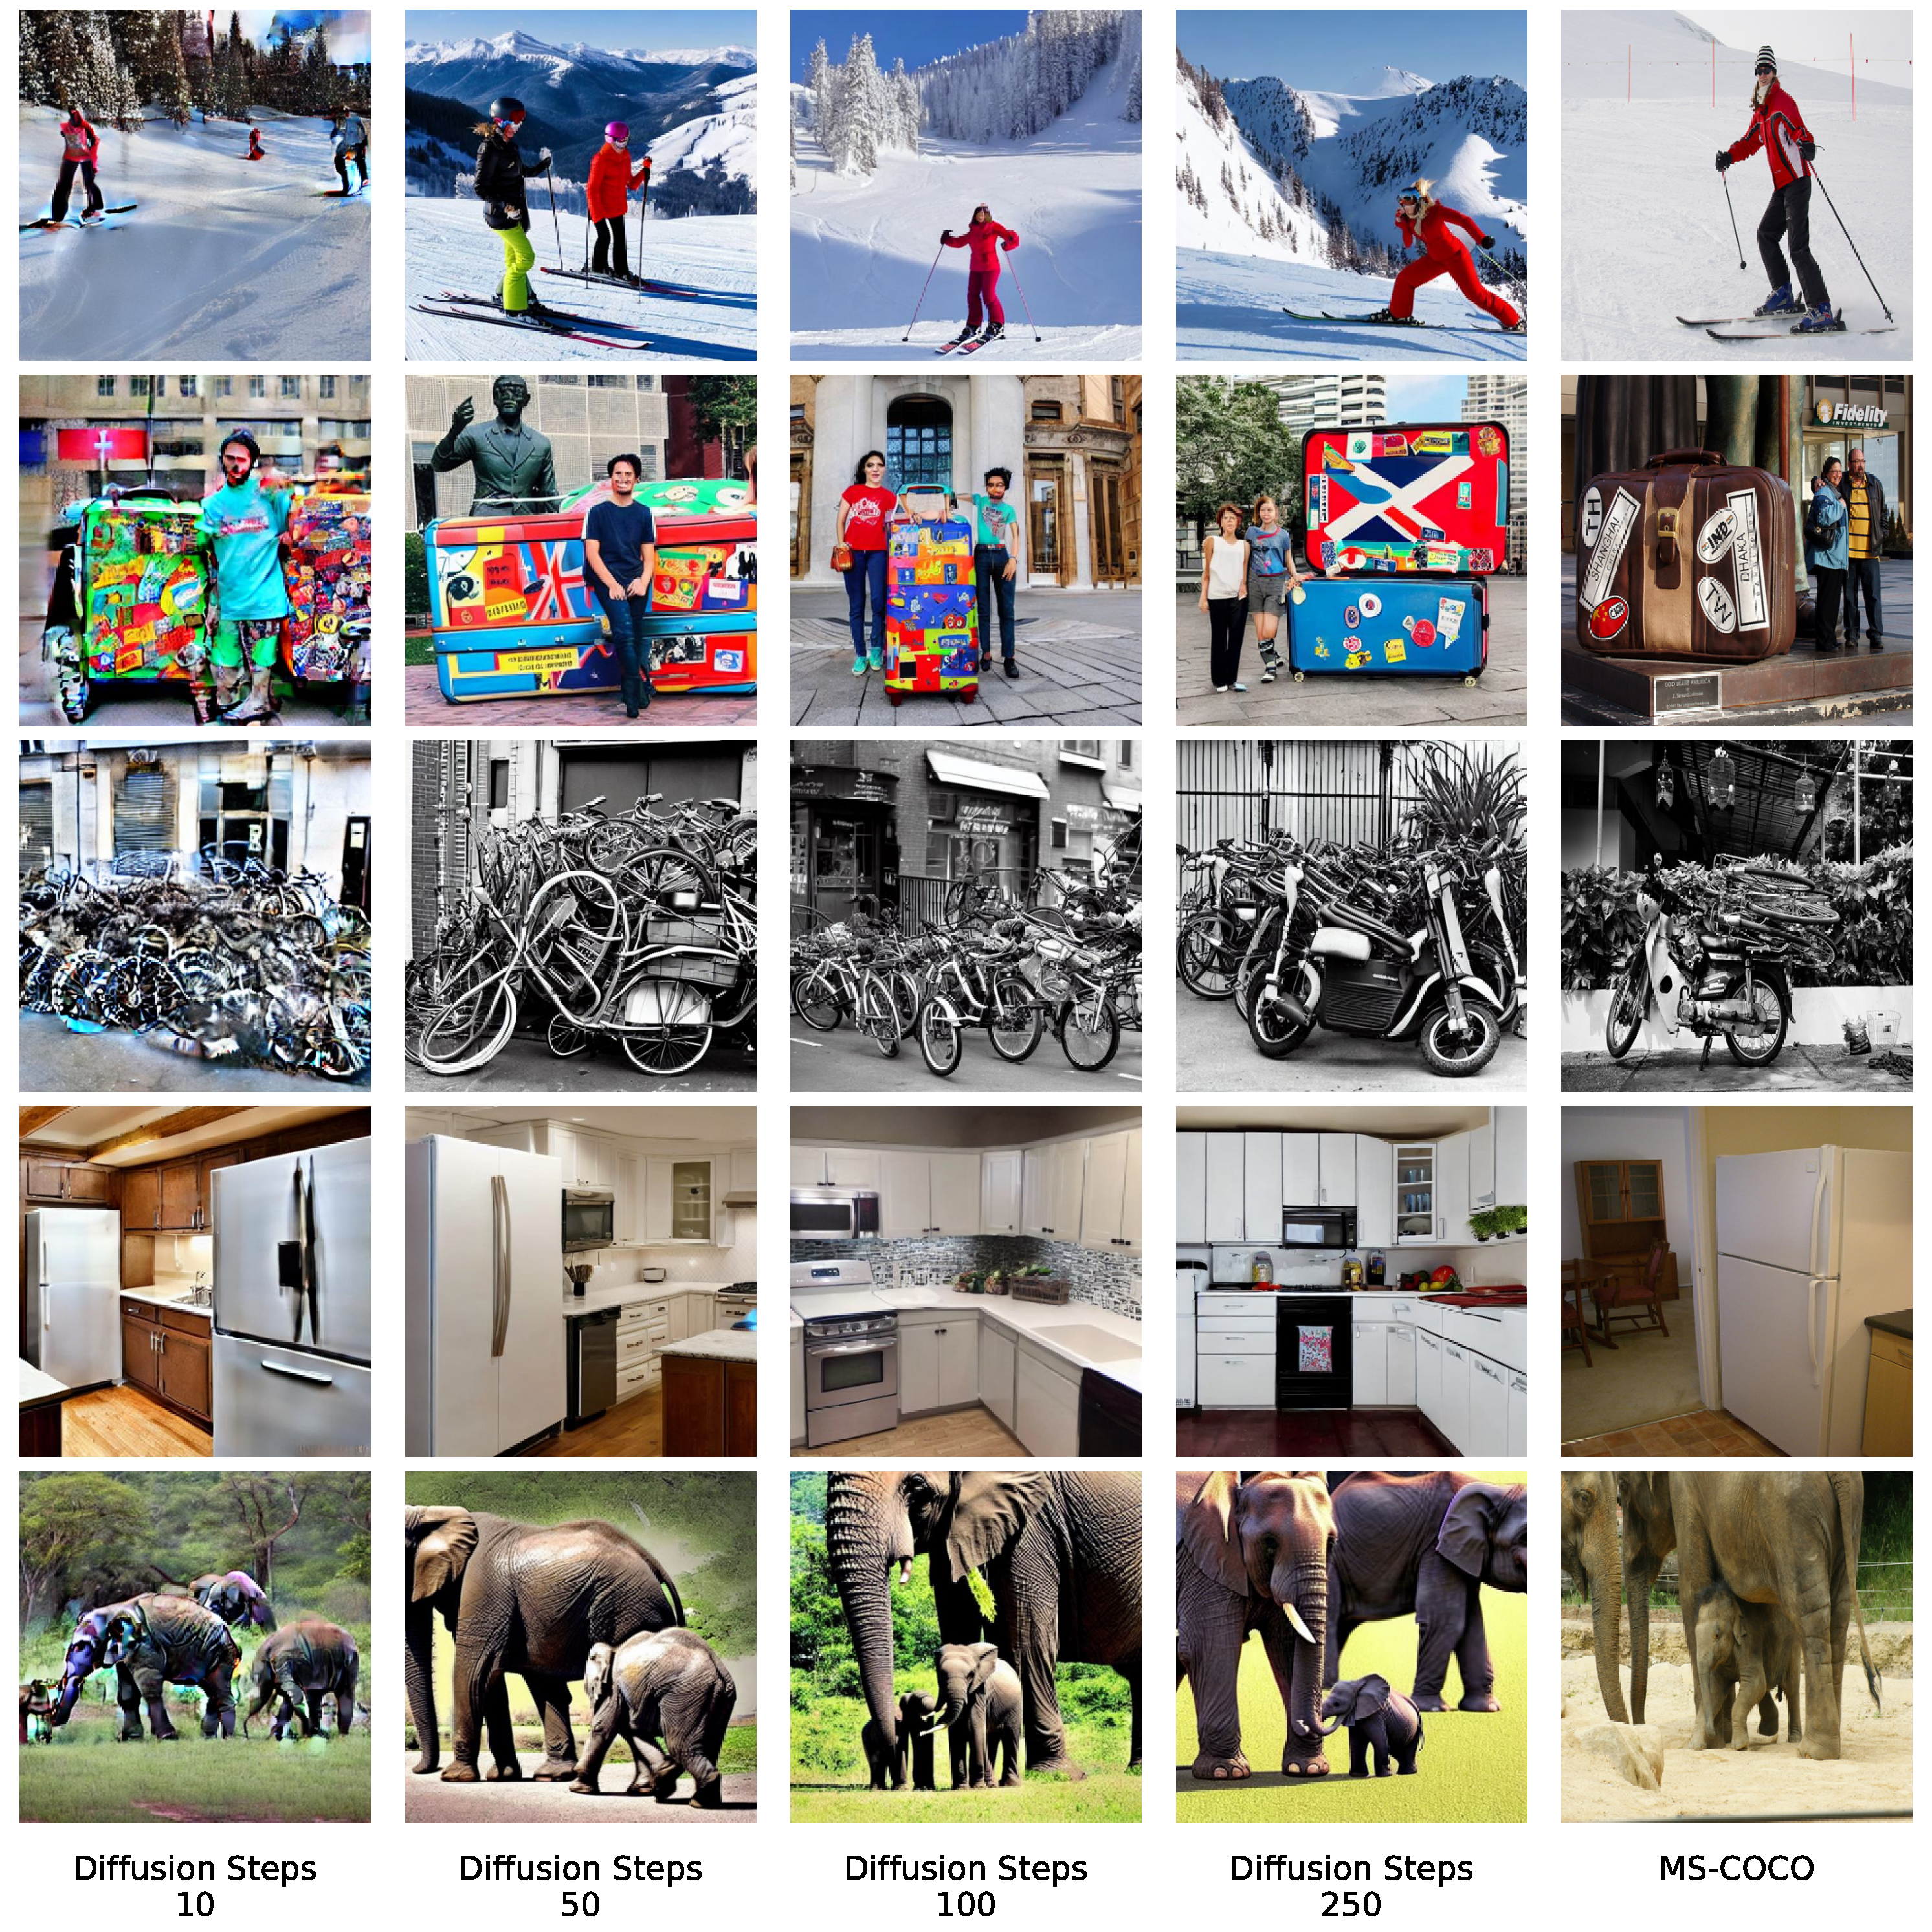
\includegraphics[width=0.8\textwidth]{assets/ddms_image_comparison.pdf}
    \caption{Generated images with different numbers of diffusion steps. On the right, the reference image from the MS-COCO dataset. The prompts where (1) \textit{A woman standing on skiis while posing for the camera.} (2) \textit{Suitcase sitting on the ground with stickers from various countries on it.} (3) \textit{Black and white photo of a scooter carrying numerous bikes.} (4) \textit{A corner of a kitchen with a big fridge.} (5) \textit{A small elephant walks underneath a big elephant.}}
    \label{fig:ddms_image_comparison}
\end{figure}

\subsection{PickScore for W\"urstchen}
In their experiments, Pernias et al.~\cite{pernias2024wrstchen} are able to show
that their method yields a significant upgrade in computational costs and in
training time, which sits at a $8\times$ reduction compared to Stable Diffusion
2.1~\cite{rombach2023sd_2_1}. Another goal of the paper is to keep the level of
image complexity. In order to compare the level of complexity to other models,
Pernias et al. picked several evaluation methods. They used the metrics
Fr\'echet Inception Distance~\cite{heusel2018ganstrainedtimescaleupdate} (see
Section~\ref{sec:experiments:stabel_diffusion:selction_of_fid}), the Inception
Score~\cite{ding2021cogviewmasteringtexttoimagegeneration}, and the human preference imitating
PickScore. Furthermore, they conducted a study with human participants. All were
given a text-prompt and the images of W\"urstchen and another model to compare.
In experiments Pernias et al. found that W\"urstchen is capable to keep up or
even succeed over models of the same dimensions. While working with W\"urstchen
we found to W\"urstchen to perform worse than presented by the authors. Thus, we
conduct experiments of the PickScore~\cite{Kirstain2023PickaPicAO} to
prove the correctness of our own suspicion. In this section, we first describe
the workingw of PickScore, then we present the setup of our experiments and
after demonstrating our results we provide a discussion.

\subsubsection{PickScore}
%
\subsubsection{Experiment description}
\subsubsection{Results}
\subsection{The Average Human Rating of ControlNet}
\subsubsection{User Study}

We conducted a user study to evaluate the performance of ControlNet compared to PITI~\cite{wang2022pretrainingneedimagetoimagetranslation} in generating images from hand-drawn sketches. Unlike the original ControlNet study~\cite{zhang2023addingconditionalcontroltexttoimage}, which included Sketch-Guided Diffusion (SGD)~\cite{voynov2022sketchguidedtexttoimagediffusionmodels} and a lighter version of ControlNet (ControlNet-lite), we were limited to PITI and ControlNet because the authors of SGD did not provide a model, and retraining it was not feasible. Additionally, the ControlNet-lite model was unavailable. In the original paper the authors mention both, Stable Diffusion (SD) V1.5 and Stable Diffusion V2 as backbones for ControlNet. However, they do not indicate which version of Stable Diffusion is used for the experiment. As the authors official GitHub "https://github.com/lllyasviel/ControlNet" contains the setup instructions for ControlNet + SD V1.5 and we could not find any indication of Stable Diffusion V2, we opted for SD V1.5 for our experiment. Furthermore, unlike PITI, which was trained on the MS-COCO dataset~\cite{lin2015microsoftcococommonobjects} only including photos, ControlNet can also generate images in different styles, i.e.\ cartoons and paintings, due to the fact that SD V1.5 was trained on the LAION-400M dataset \cite{schuhmann2021laion400mopendatasetclipfiltered}. While the original experiments goal was to evaluate the methods performance on sketch inputs only (wihtout prompts), we also evaluate the difference of ControlNets images generated with simple prompts and with no prompts, because without prompts ControlNet may produce stylized outputs. We use the prompt \textcolor{red}{``INSERT PROMPT HERE''}, as it does not hint at specific objects of the image but implicitly tells ControlNet to generate high quality, non-stylized images. 
% The ranking of images without stylization 

For this study, we sampled 20 unseen hand-drawn sketches and used them to generate images with PITI, ControlNet and ControlNet + prompt. We recruited \textcolor{red}{NUMBER OF USERS} users to rank each generated image based on two criteria: “the quality of displayed images” and “the fidelity to the sketch,” following a protocol similar to the original study. Participants ranked each image on a scale from 1 to 5, where lower scores indicate worse performance, resulting in \textcolor{red}{120 / NUMBER OF RANKINGS} rankings for each criterion (quality and fidelity).

To quantify user preferences, we computed the Average Human Ranking (AHR) for both metrics, which served as a comparative measure of how well each model adhered to the sketches and the overall image quality. Due to the constraints in model availability, our study focused on comparing the performance of PITI and ControlNet, without including comparisons with SGD and ControlNet-lite.


\newpage

\section{Societal Impacts}
The capabilities of the mentioned text-to-image models are already extraordinary, but the development did not stop with Würstchen. The quality of image generation has been further improved\cite{lin2023designbenchexploringbenchmarkingdalle} and other capabilities have been added in so-called multimodal models\cite{yasunaga2022retrievalaugmentedmultimodellanguagemodeling}. With this powerful new technology, one might immediately ask where these text-to-image models are being used today, and what side effects their use has on different groups of people.

\subsection{Application in professional contexts}
The most evident impact may be on those who work as professional artists. In 2023, researchers in Korea conducted a survey of 28 professionals working in a variety of artistic fields, from sculpture to video editing\cite{ko2023largescaletexttoimagegenartionmodelsforvisualartists}. 12 of them mentioned that Stable Diffusion and its descendants are useful for generating more reference material, which they mainly use to learn by observing what and how others create and to get inspiration for new ideas. But most of them also said that it wouldn't change their basic working paradigm. Another use case for them was rapid prototyping to enable real-time communication with their clients or artists in different fields. In addition, the artists found that the models had almost no bias in the creation of art, which made it possible to quickly create unconventional images, but also resulted in a lack of ability to personalize the results. They also said that using text-to-image technology limited their creativity because the generated images were influenced only by the text prompt, and text can never fully and accurately describe and image what the artist has in mind. This often made it frustrating to use image-generating AI in their daily work. Despite their shortcomings, it was noted that, text-to-image technologies are supporting professional artists and provide numerous opportunities.

In addition to artists, professionals in other fields are also using Stable Diffusion-like AI. Nowadays, it is easier than ever to create good to great images that you have in mind. The trend can be called "democratization of art". A Finnish study of game industry professionals\cite{vimpari2023texttoimagegenerationaibygameprofessionals} titled "An Adapt-or-die Type of Situation" explores all kinds of different ways this new technology is impacting the industry. Many of the participants were experiencing a fundamental change in their role. A third were using it daily, and another third weekly. Many of the participants, similar to the Korean artists, used AI mainly for prototyping and ideation. In architecture\cite{sekban2022artandarchtitecture}, too, text-to-image models can be used to generate design alternatives, for example, to make a design more energy efficient or sustainable. Education has also emerged as an area where image-generating AI can be applied\cite{vartiainen2023aiincraftseducation}. Again, it is used for ideation, but also as a way for children to externalize their ideas and concepts. Although it was also pointed out that the use of text-image models in the classroom poses several challenges, for example the question of what to assess when grading a student's work, as substantial parts could have been done by the AI. Even in tourism, applications are possible. According to a Chinese study\cite{miao2023aiintourism}, these AI tools have the chance to improve the anticipation, on-site and recollection experience of tourists.

What we have presented is just the peak of many professional applications of Stable Diffusion and its descendants, and we have not yet started with the private use cases. In general, we were able to identify three main applications: final image creation, ideation and prototyping.

\subsection{Risks and Concerns}
Despite all these great opportunities and applications, it is undeniable that there are risks and negative impacts of the boom of this technology.

As it becomes easier than ever to create convincing images, deepfakes are gradually becoming a significant issue. On March 22, 2023, a Twitter post went viral claiming that there had been an explosion at the Pentagon in Washington DC. The post included an AI-generated image. The fake news was allegedly spread by, among others, the Russian broadcaster "Russia Today"\cite{correctiv2023pentagonexplosion}. Posts like this are becoming more realistic and easier to produce. S. Neupane and other researchers from Mississippi State University\cite{neupane2023impactsriskgenerativeai} classify misinformation as one of the five main new attack vectors leveraging artificial intelligence.

A serious concern is the bias that these models impose on the images they generate. In general, image generation models can only reproduce what they have seen in training. This means that underrepresented data will rarely be reproduced. The consequences can be severe. A study by Microsoft\cite{naik2023socialbiasesthroughtexttoimage} showed that 70\% of the people generated by stable diffusion were white. Also, women are either largely underrepresented or overrepresented, most likely in order to avoid this problem. Another notable finding was that when generating images to the prompt "Office in Ethiopia", both DALL-E and Stable Diffusion depict Ethiopia as being in a state of poor economic conditions, while when actually looking for real images, we can clearly deduce that they are closer to offices you might see in Western countries.

Another consequence of the underrepresentation of the Global South is usability issues. In a collaboration of computer scientists from the US, Canada, and Bangladesh\cite{mim2024impactoftexttoimagetoolsinglobalsouth}, a survey of Bangladeshi image practitioners was conducted. It was found that Bangladeshis had problems creating the text prompts. To quote one of their participants \textit{"Text-based prompts need proficiency in English nouns and adjectives to explain the idea of an image to the GAI [Generative AI] system to receive an outcome that matches the image practitioner's imagination."} Another participant complained that certain Bangla words did not have an accurate English translation, in this case she wanted to describe a certain type of rain. In addition, the participants are often poorly educated, so even if text prompts were available in their native language, they wouldn't be able to accurately articulate their perception of the image. Additionally, most of the participants rely on the use of free image creation technology, as traditional, more professional applications such as \textit{Adobe Photoshop} or \textit{Adobe Illustrator} are out of reach or financially unfeasible. The study also noted the impact of the underrepresentation of data from the Global South. They asked Midjourney to depict a future version of the Gawsia market, which resulted in an image where neither the architectural features nor the physical appearance of the people matched those typically seen in Dhaka.

Furthermore, when using generated images in commercial contexts, one question that has not yet been answered is the question of copyright. Who owns a generated image? There are many possible answers to this question: The artists who created the training data, the company that trained the text-to-image model, or the user who created the text prompt. Currently, there are numerous lawsuits on this issue. Most notably, Getty Images (a leading global stock photography and media company) has sued Stability AI (the company behind Stable Diffusion), accusing them of improperly and unlawfully using millions of its copyrighted images to train Stable Diffusion models without permission\cite{cnn2023gettyimagesvsstabilityai}.

\subsection{Summary}

The rapid advancement of text-to-image models, as exemplified by Würstchen and its successors, has had a profound impact across multiple industries. These models have contributed valuable applications to professional fields such as art, architecture, education, and tourism, enabling new ways of ideation, prototyping, and final image creation. Perhaps most importantly for the creative industries, the democratization of art - now more people can easily create high-quality images - is a tectonic shift in the creative industries, empowering professionals and amateurs alike.

These benefits are accompanied by significant risks and challenges, with deepfakes, bias reinforcement in generated content, and underrepresentation of the Global South in training data raising a number of ethical and practical concerns. In addition, the ambiguity of copyright ownership in AI image generation creates legal issues that have yet to be resolved.

It's critical that these issues be addressed in the future to maximize the benefits and minimize the harms as text-to-image technology evolves. Ongoing research, ethical considerations, and regulatory frameworks will shape the positive and negative impacts of this powerful technology on society.

\section{Conclusion}
In this paper, we looked into three different works on diffusion models. First,
we explored how Stable Diffusion's~\cite{rombach2022stablediffusion}
performance boost enables feasible image generation on a larger scale by
leveraging the latent space rather than working directly in pixel space. We
reconducted the FID score experiment, which confirmed that the results of
Rombach et al.~\cite{rombach2022stablediffusion} are reproducible, indicating a
well-conducted experiment. Additionally, we examined the details and behavior
of the FID score~\cite{heusel2018ganstrainedtimescaleupdate}, proposing an
improved version, though further research is needed to fully understand its
behavior especially concerning generalization.

Secondly, we investigated W\"urstchen~\cite{pernias2024wrstchen}, which promises
to improve training efficacy of latent diffusion models while keeping or
improving the image quality with latent diffusion models of the same dimensions.
Based on our own perception, we stated the hypothesis that W\"urstchen performs
worse than the PickScore calculated by Pernias et al. indicates.
Our results confirm our suspicion as the preference of W\"urstchen is lower
than demonstrated by Pernias et al.~\cite{pernias2024wrstchen}, while still within 
range to align with their conclusion to maintain a level of image quality comparable
with other latent diffusion models of the same size. To get accurate,
reproducible results, we recommend multiple iterations of the experiments.

Thirdly, we conducted a study with human participants to compare
ControlNet's~\cite{zhang2023addingconditionalcontroltexttoimage} ability to
generate images from sketches with
PITI~\cite{wang2022pretrainingneedimagetoimagetranslation}. We focused on how
prompts, sketch fidelity, and training data impact image quality and user
preferences. ControlNet outperformed PITI in image quality, achieving
better average results, while PITI excelled in sketch fidelity, though at the
expense of overall quality. Furthermore, adding prompts to ControlNet improved
image realism without affecting sketch adherence. ControlNet's versatility in
generating various styles stems from its training on the
LAION-400M~\cite{schuhmann2021laion400mopendatasetclipfiltered} dataset.
Finally, we observed significant variability in user preferences, likely due to
subjective factors, as some participants were more sensitive to fidelity and
others to quality, influenced by their profession and AI experience.

Lastly, we analyze the societal impact of latent diffusion models. These
text-to-image models are transforming a variety of industries, from game design
to tourism. However, these models also present challenges for certain regions
and demographics, raising important questions such as those surrounding
copyright.

\newpage
\bibliographystyle{unsrt}
\bibliography{references}
\end{document}
